\documentclass[10pt,a4paper]{article}

\usepackage[english,francais]{babel}
\usepackage[utf8]{inputenc}
\usepackage{amsmath}
\usepackage{graphicx}
\usepackage[colorinlistoftodos]{todonotes}
\usepackage{caption}
\usepackage{url}
\usepackage{fancyhdr}
\usepackage{lastpage}
\usepackage{a4wide} 
\usepackage{amssymb} 
\usepackage{color}
\usepackage{fancybox}
\usepackage{moreverb}
\usepackage{listings}
\usepackage{placeins}
\usepackage{setspace}
\onehalfspacing

\title{Rapport de Stage}
\author{MONSINJON Sam}
\date{\today}

\pagestyle{headings}

\begin{document}
\lstset{ numbers=left, tabsize=3, frame=single, numberstyle=\ttfamily, basicstyle=\footnotesize} 
\thispagestyle{empty}

\begin{center}
\makebox[\textwidth][l]{
\raisebox{-8pt}[0pt][0pt]{
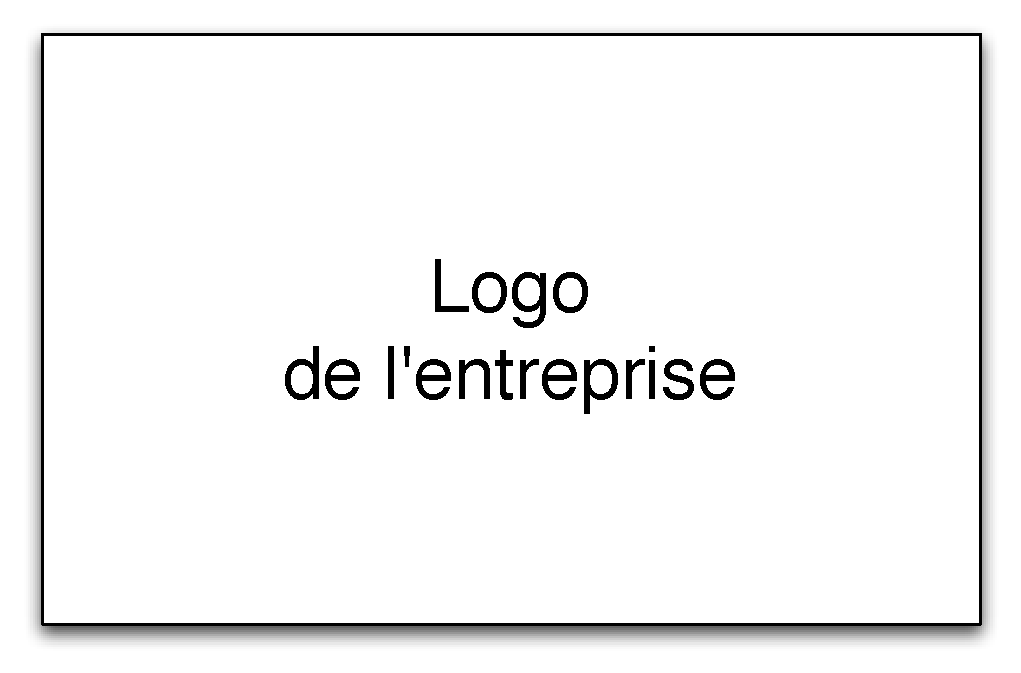
\includegraphics[scale=0.18]{logo_entreprise.pdf}
}
}
\makebox[\textwidth][r]{
\raisebox{0pt}[0pt][0pt]{

\includegraphics[scale=0.2]{logo_ensimag.pdf}
}
}
Grenoble INP  -- ENSIMAG\\
École Nationale Supérieure d'Informatique et de Mathématiques Appliquées\\
\vspace{3cm}
{\LARGE Rapport de Stage}\\
\vspace{1cm}
Effectué chez SILEX TECHNOLOGIES\\
\vspace{2cm}
\shadowbox{
\begin{minipage}{1\textwidth}
\begin{center}
{\Huge Implémentation de payoffs de produits structurés}\\
\end{center}
\end{minipage}
}\\
\vspace{3cm}
MONSINJON Sam\\
2e année -- Option IF\\
\vspace{3mm}
17 Juin 2019 -- 23 août 2019\\
\vspace{4cm}
\begin{tabular}{p{10cm}p{10cm}}
{\bf Nom Entreprise}                                            &{\bf Responsable de stage}\\
{\footnotesize Adresse Entreprise}       & ~~~Nom Et Prénom Tuteur Entreprise\\
{\footnotesize BP XX}                                        & {\bf Tuteur de l'école}\\
{\footnotesize 38000 Grenoble Cedex}                          & ~~~Nom et PrénomTuteur Ecole\\
\end{tabular}
\end{center}

\newpage
\tableofcontents
\newpage
\section{Introduction}
Du 17 juin 2019 au 23 août 2019, j'ai eu la chance d'effectuer un stage assistant ingénieur au sein de SILEX, une société de gestion d'actifs financiers. Lors de ce stage, je me suis retrouvé au sein du pôle technologique, et j'ai eu pour principale mission de travailler sur un priceur de produits structurés.

Plan du rapport




\newpage

\section{SILEX}
\subsection{Présentation globale}
SILEX est une société de gestion d'actifs créée en 2016. L'entreprise est divisée en trois principales entités : 
\begin{itemize}
    \item SILEX AM : Ce pôle s'occupe de la gestion d'actifs des clients de la société, qui sont principalement des gérants de fortune.
    \item SILEX FINANCE : Ce pôle est constitué de vendeurs. à développer% Ceux-ci vendent en particulier des produits structurés.
    \item SILEX TECHNOLOGIES : Ce pôle, dans lequel je travaillais pendant mon stage, est un pôle de recherche \& développement. Celui-ci s'occupe principalement d'implémenter des outils qu'utilisent les vendeurs et les gerants de portefeuilles, en particulier l'outil SPARK, utilisé par les gérants de portefeuilles.
\end{itemize}
 \subsection{L'outil SPARK}
 La technologie SPARK est un outil développé par les ingénieurs de SILEX technologies. SPARK est utilisé pour aider les gérants de portefeuilles à construire, optimiser et suivre un portefeuille. Il y a pour le moment, deux versions de SPARK : \textit{STOCKS ALLOCATOR} qui se concentre exclusivement sur le marchés des actions, et \textit{ASSET ALLOCATOR} qui concerne plusieurs types de produits (actions, obligations, ETF etc...).  \vspace{0.5em}
 
 Bien que je n'ai pas travaillé sur cet outil lors de mon stage, il est important de le mentionner dans ce rapport car SPARK est l'un des principaux atout de SILEX. De plus, le projet sur lequel j'ai travaillé va, à terme, intégré cet outil.

\newpage
\section{Problématique}
\newpage
\section{Résolution}
\newpage
\section{Résultats}
\newpage
\section{Bilan}
\newpage
\section{Bibliographie}

Ci-dessous une collection de références vers les différentes ressources m'ayant servi lors de la réalisation de ce projet personnel en humanités.\\\\

Vidéos TED sur les jeux vidéo :

\begin{thebibliography}{0}
    \bibitem{GabeZichermann} Gabe \textsc{Zichermann}. \emph{How games make kids smarter}. TEDxKids@Brussels, filmé en Juin 2011 (consulté le 12 Décembre 2015). Disponible sur :\\ \url{http://www.ted.com/talks/gabe_zichermann_how_games_make_kids_smarter}
     \bibitem{JaneMcGonigal} Jane \textsc{McGonigal}. \emph{Gaming can make a better world}. TED2010, filmé en Février 2010 (consulté le 12 Décembre 2015). Disponible sur :\\ \url{http://www.ted.com/talks/jane_mcgonigal_gaming_can_make_a_better_world}
     \bibitem{DaphneBavelier} Daphne \textsc{Bavelier}. \emph{Your brain on video games}. TEDxCHUV, filmé en Juin 2012 (consulté le 12 Décembre 2015). Disponible sur :\\ \url{http://www.ted.com/talks/daphne_bavelier_your_brain_on_video_games}\\\\
\end{thebibliography}

Et quelques sites internet :

\begin{thebibliography}{0}
    \bibitem{HuffPost} David \textsc{Freeman}. \emph{Violent Video Games May Curb Bullying In Vulnerable Children, Study Suggests}. The Huffington Post, écrit le 28 Août 2013 (consulté le 01 Décembre 2015). Disponible sur :\\ \url{http://www.huffingtonpost.com/2013/08/28/violent-video-games-bullying-children-study_n_3823490.html}
     \bibitem{MotherJones}  Erik \textsc{Kain}. \emph{The Truth About Video Games and Gun Violence}. The Huffington Post, écrit le 11 Juin 2013 (consulté le 01 Décembre 2015). Disponible sur :\\ \url{http://www.motherjones.com/politics/2013/06/video-games-violence-guns-explainer}
\end{thebibliography}

\newpage

\section{ANNEXES}

\subsection{Rapport du questionnaire}

\end{document}